\subsection{Джойстик и приемник}

Използван е джойстик за управление \textit{Dx6i} на \textit{Spektrum} (\autoref{fig:spectrum_joystick}).
Джойстикът има 6 канала
и се свързва към  приемника чрез радиовълни с честота \(2.4GHz\), използвайки
технология, разработена от производителя и наречена \textit{DSM Spread Spektrum Technology}.
Затова се налага използването на приемник, който поддържа специфичната технология.

\begin{figure}[htpb!]
    \centering
    
\includegraphics[width=0.6\textwidth]{spectrum_joystick}
    \caption{Джойстик Spektrum Dx6i}
    \label{fig:spectrum_joystick}
\end{figure}

Използван е приемник \textit{AR6200} на \textit{Spektrum} (\autoref{fig:spectrum_reciever_img}), който поддържа \textit{DSM Spread Spektrum Technology} на джойстика.
Каналите на изходите предоставят ШИМ сигнал с честота \(50Hz\) и запълване в диапазона \(9500\to1950 \mu s\).


\begin{figure}[htpb!]
    \centering
    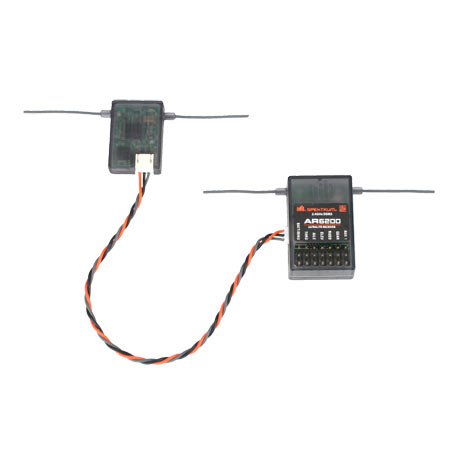
\includegraphics[width=0.6\textwidth]{spectrum_reciever_img}
    \caption{Приемник AR6200}
    \label{fig:spectrum_reciever_img}
\end{figure}

Като конфигурацията на изходните пинове на приемника е описана в \autoref{fig:reciever_wires}.

\begin{figure}[htpb!]
    \centering
    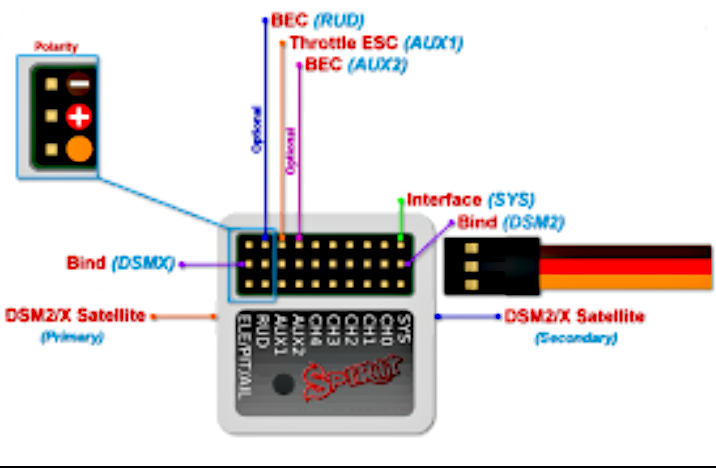
\includegraphics[width=0.8\textwidth]{reciever_wires}
    \caption{Диаграма за свързване на изходните пинове на приемника}
    \label{fig:reciever_wires}
\end{figure}



\FloatBarrier
